\documentclass[12pt]{article}


\usepackage[top=2cm,bottom=2cm,left=2cm,right=2cm]{geometry}
\usepackage[pdftex]{graphicx} %per poter inserire le figure\label
\usepackage{amssymb,amsmath,amsthm,amsfonts}
	%\numberwithin{equation}{chapter}
\usepackage{xspace}
\usepackage{tabularx}
\usepackage{indentfirst}
%\usepackage{subfigure}
\usepackage[small]{caption}
\usepackage{eucal}
\usepackage{eso-pic}
\usepackage{url}
\usepackage{booktabs}
\usepackage{afterpage}
\usepackage{parskip}
\usepackage{listings}
\usepackage{fancyhdr}
\usepackage{textcomp}
\usepackage{cite}
\usepackage{multirow}
\usepackage[utf8]{inputenc}   %per riuscire a scrivere gli accenti
%\usepackage[italian]{babel}   %per riuscire a scrivere gli accenti
\usepackage{setspace}
\usepackage{listings}

\usepackage{subfig}

\usepackage{xcolor}
\usepackage{array} 
\usepackage{graphicx}
\usepackage[colorinlistoftodos]{todonotes}
\usepackage{wrapfig}
\usepackage{float}
\usepackage[export]{adjustbox}
\usepackage{makeidx}
\usepackage{siunitx}
\usepackage[bookmarks=true]{hyperref}

\setlength {\marginparwidth }{2cm}


\definecolor{vgreen}{RGB}{104,180,104}
\definecolor{vblue}{RGB}{49,49,255}
\definecolor{vorange}{RGB}{255,143,102}

\lstdefinestyle{verilog-style}
{
    language=Verilog,
    basicstyle=\small\ttfamily,
    keywordstyle=\color{vblue},
    identifierstyle=\color{black},
    commentstyle=\color{vgreen},
    numbers=left,
    numberstyle=\tiny\color{black},
    numbersep=10pt,
    tabsize=8,
    %moredelim=*[s][\colorIndex]{[}{]},
    %literate=*{:}{:}1
}

\begin{document}


\begin{titlepage}

\center 

{\large \today}\\[2cm] 

\textsc{\LARGE Università degli Studi di Padova}\\[1.5cm]


\textsc{\Large Hardware implementation \\ of base 2 logarithm}\\[0.5cm] 


\begin{minipage}{0.4\textwidth}
\large
\emph{Authors:} \\
Gabriele \textsc{Bortolato} \\
\end{minipage}

\vfill 

\end{titlepage}

\section{Methods}
\subsection{Look-up table}
Given an integer input $x$ (from $0$ to $2^{64}-1$), this method follows three steps:
\begin{itemize}
    \item find the MSB position of $x$ with a priority encoder ($PE_{out}$) 
    \item compute the 'rest' ($r$)
    \item rest is converted to the fraction part of the logarithm with a look-up table (LUT) 
\end{itemize}
Once the fractional width is selected the LUT output can be computed; greater the fractional width grater the precision of the results, but higher will be the resources requirement.  

The MSB position is extracted with a priority encoder shown below. 

\begin{equation}
    PE_{out} = \log_2{x}
\end{equation}

\begin{lstlisting}[style={verilog-style}]
always @(posedge clk)   // Priority encoder
begin
    if      (x[63]) prienc <=   6'd63;
            //                  //
            //                  //
    else if (x[2])  prienc <=   6'd2;
    else if (x[1])  prienc <=   6'd1;
    else            prienc <=   6'd0;
end
\end{lstlisting}

Secondly the rest is computed and its width is matched with the LUT input width.

\begin{equation}
    r=x-2^{PE_{out}}
\end{equation}  
 

\begin{lstlisting}[style={verilog-style}]
r <= ((x-(16'b1<<prienc))<<(IN_W-prienc)>>IN_W-F_W));
\end{lstlisting}

Finally this rest is injected to the precomputed LUT and the fractional part is found.

\begin{equation}
    frac=LUT(r)
\end{equation}

\begin{lstlisting}[style={verilog-style}]
case(r)     // frac = LUT [r]
    10'd0:frac  <= 10'd0;
    10'd1:frac  <= 10'd1;
        //      //   
        //      //  
    10'd1022:frac   <= 10'd1023;
    10'd1023:frac   <= 10'd1023;
endcase
\end{lstlisting}

Finally the result is obtained with a simple sum.

\begin{equation}
    \log_2{x}=PE_{out}+\frac{frac}{2^{frac \_ width}}
\end{equation}

\begin{lstlisting}[style={verilog-style}]
y <= (prienc<<F_W) + frac;
\end{lstlisting}

\subsection{Taylor expansion}
This method follow the same first step of the previous one, but the fractional part is computed with a Taylor expansion.
\begin{equation} 
\begin{split}
\log_2(x) & = \log_2\left(\frac{x \cdot 2^{PE_{out}}}{2^{PE_{out}}}\right) \\
 & = PE_{out} + \log_2\left(\frac{x}{2^{PE_{out}}}\right) \\
 & = PE_{out} + \log_2\left(1+r\right) \\
\end{split}
\end{equation}

Where $r$ is
\begin{equation}
    r=\frac{x-2^{PE_{out}}}{2^{PE_{out}}}\in[0,1[
\end{equation}

Now the second logarithm is computed with the following expansion.
\begin{equation}
    \log_2\left(1+r\right)=\frac{1}{\ln(2)}\left(r-\frac{r^2}{2}+\frac{r^3}{3}+ \cdot \cdot \cdot \right) 
\end{equation}

\begin{lstlisting}[style={verilog-style}]
localparam [9:0] i_ln2    = 10'd739;  // 1/(ln2) 10_fix_9
localparam [9:0] i_ln2_2  = 10'd369;  // 1/(2*ln2)
localparam [9:0] i_ln2_3  = 10'd246;  // 1/(3*ln2)

I_order_1   <= ((x-(64'b1<<prienc))<<(IN_W-prienc))>>(IN_W-F_W);
                    
I_order_2   <= I_order_1;
II_order_2  <= I_order_1*I_order_1;
                    
I_order_3   <= I_order_2;
II_order_3  <= II_order_2[2*F_W-1:F_W];
III_order_3 <= II_order_2[2*F_W-1:F_W]*I_order_2;

y_1  <= prienc<<(F_W+9);
y_2  <= y_1 + I_order_1[2*F_W-1:F_W]  *i_ln2  ;
y_3  <= y_2 - II_order_2[2*F_W-1:F_W] *i_ln2_2;
y_4  <= y_3 + III_order_3[2*F_W-1:F_W]*i_ln2_3;

\end{lstlisting}


Each correction order implies the introduction of two DSPs (multipliers) and they are limited in number, for example in the PYNQ-Z2 board (Zynq7020) 120 of them are present. 
\section{Hardware utilization}
It will be utilized a PYNQ-Z2 board for testing purposes. A DMA will be employed to transfer the data from the PS (Processing System) to the PL (Programmable Logic) and viceversa. The PL log result will be compared with the numpy PS result.  

In this example a 64 bits integer input will be fed in to the two module, the result is in fixed point format with 10 fractional bits (16\_fix\_10).


\begin{table}[h]
\begin{tabular}{c|ccccc}
Method           & FF  & LUT & BRAM & DSP & Delay [C.C.] \\ \hline
Look-up table    & 122 & 208 & 0.5  & 0   & 3 \\
Taylor expansion & 106 & 202 & 0    & 5   & 4 \\

\end{tabular}
\end{table}

As it clearly visible both methods use roughly the same amount of flip-flops and look-up tables, but the LUT method uses a BRAM block (larger the fractional width is, larger the RAM) and the expansion method uses DSPs.  
The first method has a fixed delay of a 3 clock cycles \footnote{LUT input evaluation, LUT output and adder}, instead the second method produces a delay related to the order correction \footnote{rest evaluation and one clock cycle per order correction}.


\section{PYNQ-Z2 Deploying}

\subsection{Look-up table}

In the FIG:\ref{fig:LUT_resp} is shown a 10 bits LUT response. This output is precomputed via a python script that makes use of the np.log2 and np.round numpy functions. 
\begin{figure*}[h]
    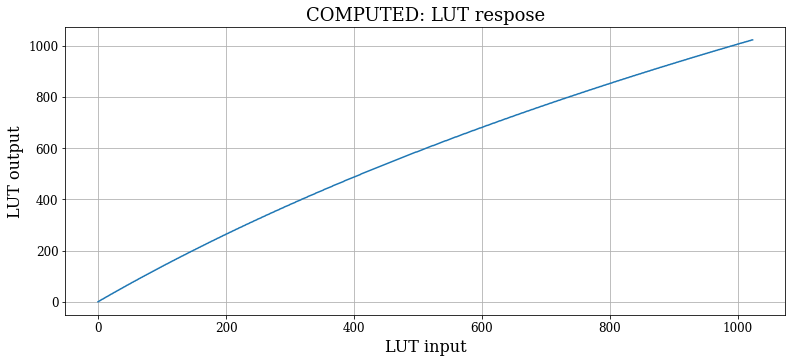
\includegraphics[width=1.0\textwidth]{Images/LUT_response.png}
    \caption{LUT employed for the fractional part. In this example a 10 bits wide LUT is employed, its value are generated by a python script.}
    \label{fig:LUT_resp}
\end{figure*}

In FIG:\ref{fig:LUT_LOG} is shown the output of $2^{20}$ random integer samples computed with np.log function and LUT method.

\begin{figure*}[h]
    \begin{minipage}[c]{0.5\linewidth}
        \vspace{0pt}
        \centering
        \subfloat[Expected module response]{
            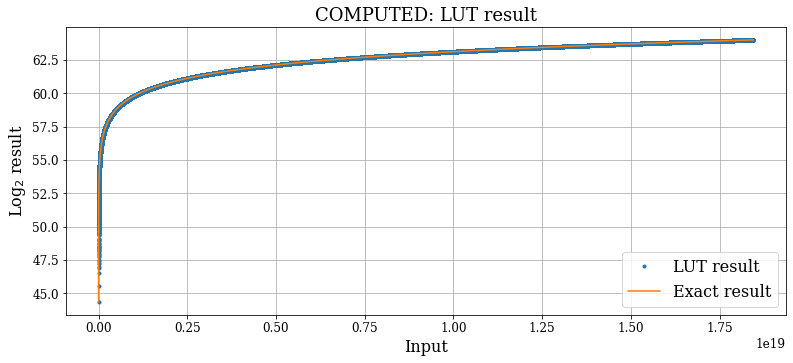
\includegraphics[height=4cm]{Images/LUT_LOG_out.png}
            \label{fig:comp_LUT_LOG}
        }
    \end{minipage}%
    \hfill%
    \begin{minipage}[c]{0.5\linewidth}
        \vspace{0pt}
        \centering
        \subfloat[Hardware implementation response]{
            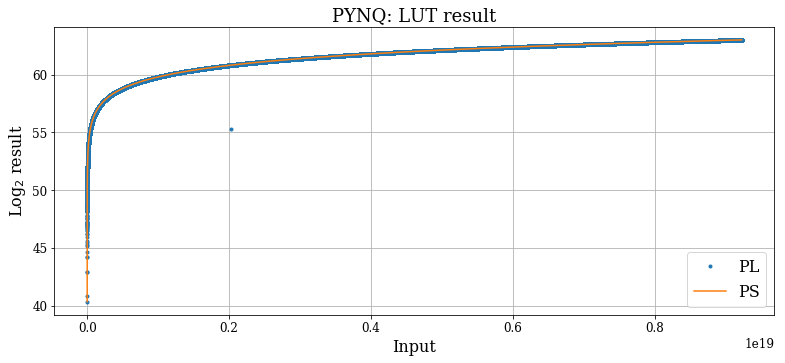
\includegraphics[height=4cm]{Images/PYNQ_LUT_res.png}
            \label{fig:PYNQ_LUT_LOG}
        }
    \end{minipage}%
    \caption{Comparisons between expected and actual "LOG LUT" module response with the exact logarithm value, in both cases $2^{20}$ random input samples are considered.}
    \label{fig:LUT_LOG}
\end{figure*}


The FIG:\ref{fig:LUT_Error} highlight the error distribution introduced by this method, the ladder depends on the rounding method used and the width selected.
\begin{figure*}[h]
    \begin{minipage}[c]{0.5\linewidth}
        \vspace{0pt}
        \centering
        \subfloat[Expected module response]{
            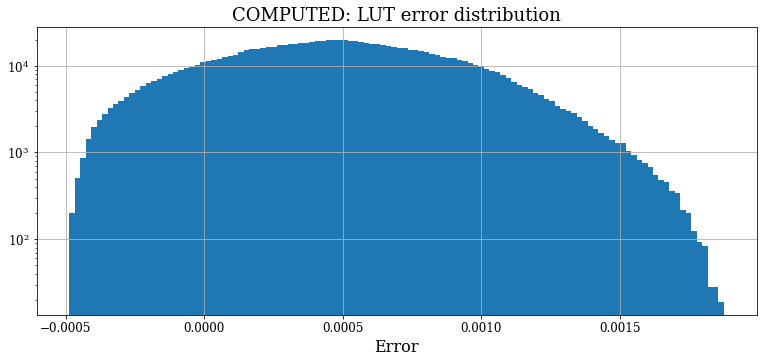
\includegraphics[height=4cm]{Images/LUT_LOG_error.png}
            \label{fig:comp_LUT_LOG_err}
        }
    \end{minipage}%
    \hfill%
    \begin{minipage}[c]{0.5\linewidth}
        \vspace{0pt}
        \centering
        \subfloat[Hardware implementation response]{
            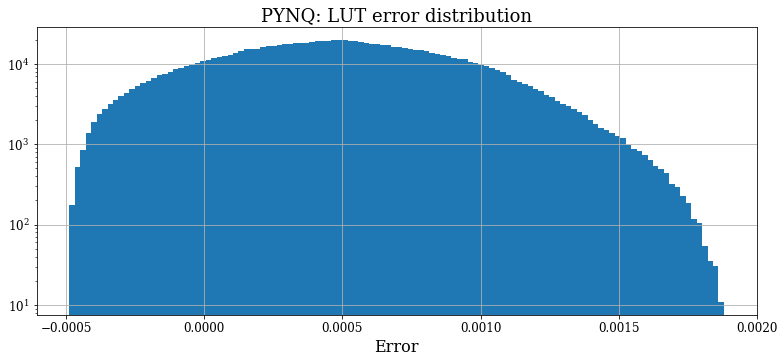
\includegraphics[height=4cm]{Images/PYNQ_LUT_LOG_error.png}
            \label{fig:PYNQ_LUT_LOG_err}
        }
    \end{minipage}%
    \caption{Error distributions.}
    \label{fig:LUT_Error}
\end{figure*}


\newpage

\subsection{Taylor expansion}

In FIG:\ref{fig:TE_resp} show the taylor expansion response in function of the input rest, it is shown the III order approximation, the average of the III order and II order and the exact response.
\begin{figure*}[h]
    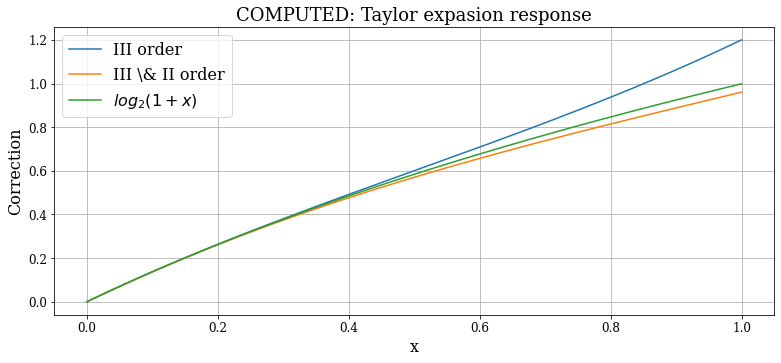
\includegraphics[width=1.0\textwidth]{Images/TE_respnse.png}
    \caption{Fractional part estimation with Taylor expansion.}
    \label{fig:TE_resp}
\end{figure*}

Similar to the previous method in FIG:\ref{fig:TE_LOG} is shown the response of the taylor expansion method, the various steps are caused by the $PE_{out}$ change.
\begin{figure*}[h]
    \begin{minipage}[c]{0.5\linewidth}
        \vspace{0pt}
        \centering
        \subfloat[Expected module response]{
            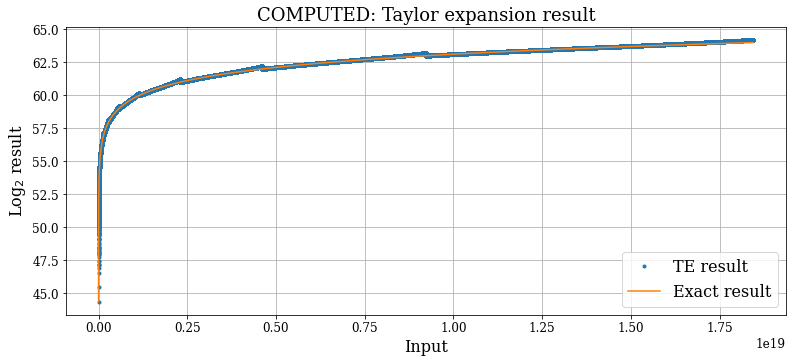
\includegraphics[height=4cm]{Images/TE_LOG_out.png}
            \label{fig:comp_TE_LOG}
        }
    \end{minipage}%
    \hfill%
    \begin{minipage}[c]{0.5\linewidth}
        \vspace{0pt}
        \centering
        \subfloat[Hardware implementation response]{
            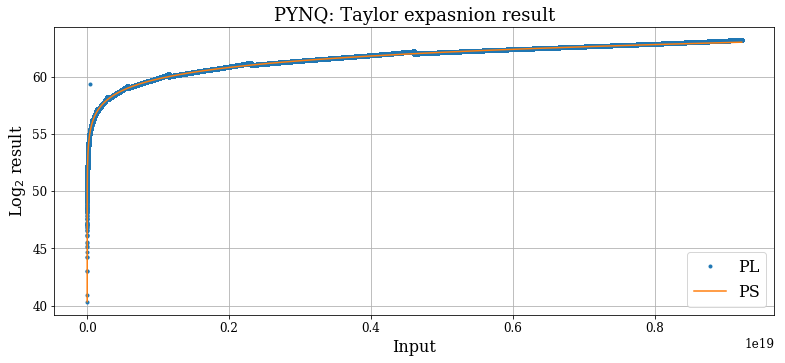
\includegraphics[height=4cm]{Images/PYNQ_TE_res.png}
            \label{fig:PYNQ_TE_LOG}
        }
    \end{minipage}%
    \caption{Comparisons between expected and actual "LOG TE" module response with the exact logarithm value, in both cases $2^{20}$ random input samples are considered.}
    \label{fig:TE_LOG}
\end{figure*}

The error distribution in FIG:\ref{fig:TE_Error} is only negative as the III order expansion is always grater than the log result (II order is always positive instead).
\begin{figure*}[h]
    \begin{minipage}[c]{0.5\linewidth}
        \vspace{0pt}
        \centering
        \subfloat[Expected module response]{
            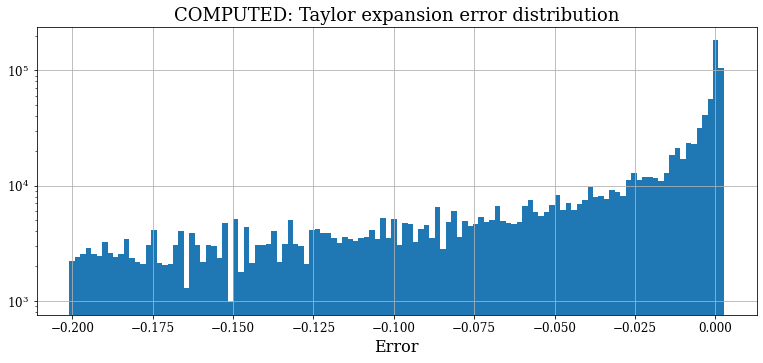
\includegraphics[height=4cm]{Images/TE_LOG_error.png}
            \label{fig:comp_TE_LOG_err}
        }
    \end{minipage}%
    \hfill%
    \begin{minipage}[c]{0.5\linewidth}
        \vspace{0pt}
        \centering
        \subfloat[Hardware implementation response]{
            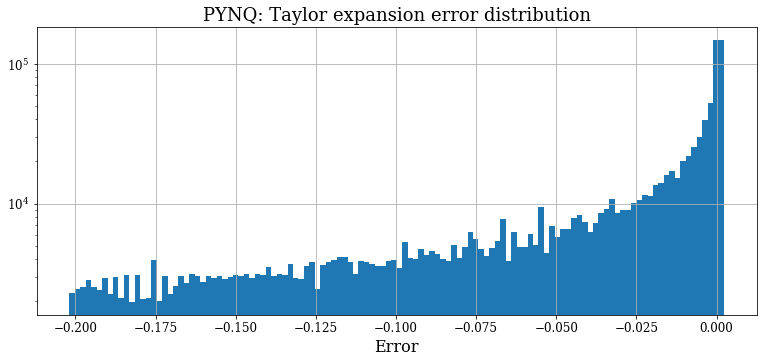
\includegraphics[height=4cm]{Images/PYNQ_TE_LOG_error.png}
            \label{fig:PYNQ_TE_LOG_err}
        }
    \end{minipage}%
    \caption{Error distributions.}
    \label{fig:TE_Error}
\end{figure*}

\subsection{Execution time}

Here a simple test is produced to evaluate the time performance of the modules.
\begin{table}[h]
\begin{tabular}{c||ccccccc} 
Method           & 10MHz  & 25MHz  & 50MHz & 100MHz & 166.67MHz & 200MHz & 250MHz\\ \hline
Look-up table    & 101ns & 41ns & 21ns & 11ns & 7ns & 7ns & FAILED\\
Taylor expansion & 101ns & 41ns & 21ns & 11ns & 7ns & 7ns & FAILED\\
\end{tabular}
\end{table}

For comparison the PS with the ARM clocked at 650 MHz produced a computation time per sample of 345 ns.

\section{Conclusions}

The errors introduced by the two methods are now presented.
\begin{table}[h]
\begin{tabular}{c||cc|cc}
&\multicolumn{2}{c|}{COMPUTED}&\multicolumn{2}{c}{PYNQ implementation} \\ \hline 
Method           & Mean error  & STD & Mean error  & STD  \\ \hline
Look-up table    & $4.9\times 10^{-4}$ & $4.1\times 10^{-4}$  & $4.9\times 10^{-4}$ & $4.1\times 10^{-4}$ \\
Taylor expansion & $-4.3\times 10^{-2}$ & $5.5\times 10^{-2}$ & $-4.3\times 10^{-2}$ & $5.6\times 10^{-2}$ \\
\end{tabular}
\end{table}
The LUT method introduces an error two order of magnitude smaller than the taylor expansion method but it requires a script to generate the LUT output, this means that it is not possible to change its parameter in the vivado framework (input width, fractional width and so on), it also uses BRAM blocks.  
The second method has the only advantage to be customizable in vivado, but it has worse performance in terms of precision and delay and it employs DSPs which are limited in number.

\end{document}